% Prof. Dr. Ausberto S. Castro Vera
% UENF - CCT - LCMAT - Curso de Ci\^{e}ncia da Computa\c{c}\~{a}o
% Campos, RJ,  2023
% Disciplina: Paradigmas de Linguagens de Programa\c{c}\~{a}o
% Aluno: Mariana Cossetti Dalfior

%%%*****************************************************************************************%%%
\chapter{ Aplica\c{c}\~{o}es da Linguagem Python}
%%%*****************************************************************************************%%%

Como foi observado nos cap\'{\i}tulos anteriores a linguagem Python pode ser aplicada de diversas maneiras. A seguir ser\'{a} apresentado algumas dessas aplica\c{c}\~{o}es.

%%%=========================================================================================%%%
	\section{Opera\c{c}\~{o}es b\'{a}sicas}
%%%=========================================================================================%%%
Em Python \'{e} poss\'{\i}vel realizar as opera\c{c}\~{o}es b\'{a}sicas de forma r\'{a}pida e pr\'{a}tica. As mais conhecidas s\~{a}o adi\c{c}\~{a}o, subtra\c{c}\~{a}o, multiplica\c{c}\~{a}o e divis\~{a}o. Elas s\~{a}o representadas da seguinte maneira: \cite{Banin2018}
   
   \begin{table}[h]
   	\centering
   	{\renewcommand\arraystretch{1.25}
   		\begin{tabular}{ l l }
   			\multicolumn{1}{p{4cm}|} {\centering\textbf{Opera\c{c}\~{o}es}} &
   			\multicolumn{1}{p{4.217cm}}{\centering\textbf{Operador}}
   			\\    
   			\cline{1-1}\cline{2-2}
   			\multicolumn{1}{p{4cm}|}{Adi\c{c}\~{a}o} &
   			\multicolumn{1}{p{4cm}}{\centering + }
   			\\  
   			\multicolumn{1}{p{4cm}|}{Subtra\c{c}\~{a}o} &
   			\multicolumn{1}{p{4cm}}{\centering -}
   			\\   
   			\multicolumn{1}{p{4cm}|}{Multiplica\c{c}\~{a}o} &
   			\multicolumn{1}{p{4cm}}{\centering * }
   			\\   
   			\multicolumn{1}{p{4cm}|}{Divis\~{a}o} &
   			\multicolumn{1}{p{4cm}}{\centering /}
   			\\   
   			\multicolumn{1}{p{4cm}|}{Divis\~{a}o inteira} &
   			\multicolumn{1}{p{4cm}}{\centering //}
   			\\   
   			\multicolumn{1}{p{4cm}|}{Resto da divis\~{a}o (m\'{o}dulo)} &
   			\multicolumn{1}{p{4cm}}{\centering \%}
   			\\  
   			\multicolumn{1}{p{4cm}|}{Potencia\c{c}\~{a}o} &
   			\multicolumn{1}{p{4cm}}{\centering **}
   			\\  
   	\end{tabular} }		
   		\caption{Opera\c{c}\~{o}es e seus operadores em Python}
   \end{table}

Essa aplica\c{c}\~{a}o \'{e} praticamente uma calculadora, em que os objetos \textsl{x} e \textsl{y} entram no c\'{o}digo com o \textsl{input} e as opera\c{c}\~{o}es ocorrem atrav\'{e}s das fun\c{c}\~{o}es pr\'{e}-definidas. Essas s\~{a}o atribu\'{\i}das a vari\'{a}vel resultado e por fim \'{e} mostrado na tela com o \textsl{print}.  A seguir \'{e} poss\'{\i}vel observar o c\'{o}digo fonte \ref{fontecalc} e o resultado \ref{resulcalc} da sua aplica\c{c}\~{a}o:
    
\begin{lstlisting}
>>> def somar(a, b):
>>> return a + b
>>> 
>>> def subtrair(a, b):
>>> return a - b
>>> 
>>> def multiplicar(a, b):
>>> return a * b
>>> 
>>> def dividir(a, b):
>>> if b != 0:
>>> return a / b
>>> else:
>>> return "Erro: divisao por zero"
>>> 
>>> print("Selecione a operacao:")
>>> print("1. Somar")
>>> print("2. Subtrair")
>>> print("3. Multiplicar")
>>> print("4. Dividir")
>>> 
>>> operacao = input("Qual operacao? (1,2,3,4): ")
>>> x = float(input("Digite o primeiro numero: "))
>>> y = float(input("Digite o segundo numero: "))
>>> 
>>> if operacao == '1':
>>> resultado = somar(x, y)
>>> print("Resultado:", resultado)
>>> elif operacao == '2':
>>> resultado = subtrair(x, y)
>>> print("Resultado:", resultado)
>>> elif operacao == '3':
>>> resultado = multiplicar(x, y)
>>> print("Resultado:", resultado)
>>> elif operacao == '4':
>>> resultado = dividir(x, y)
>>> print("Resultado:", resultado)
>>> else:
>>> print("Escolha invalida")
>>> 
\end{lstlisting}
    
    \begin{figure}[H]
    	\begin{center}
    		\caption{C\'{o}digo fonte da calculadora} \label{fontecalc}
    		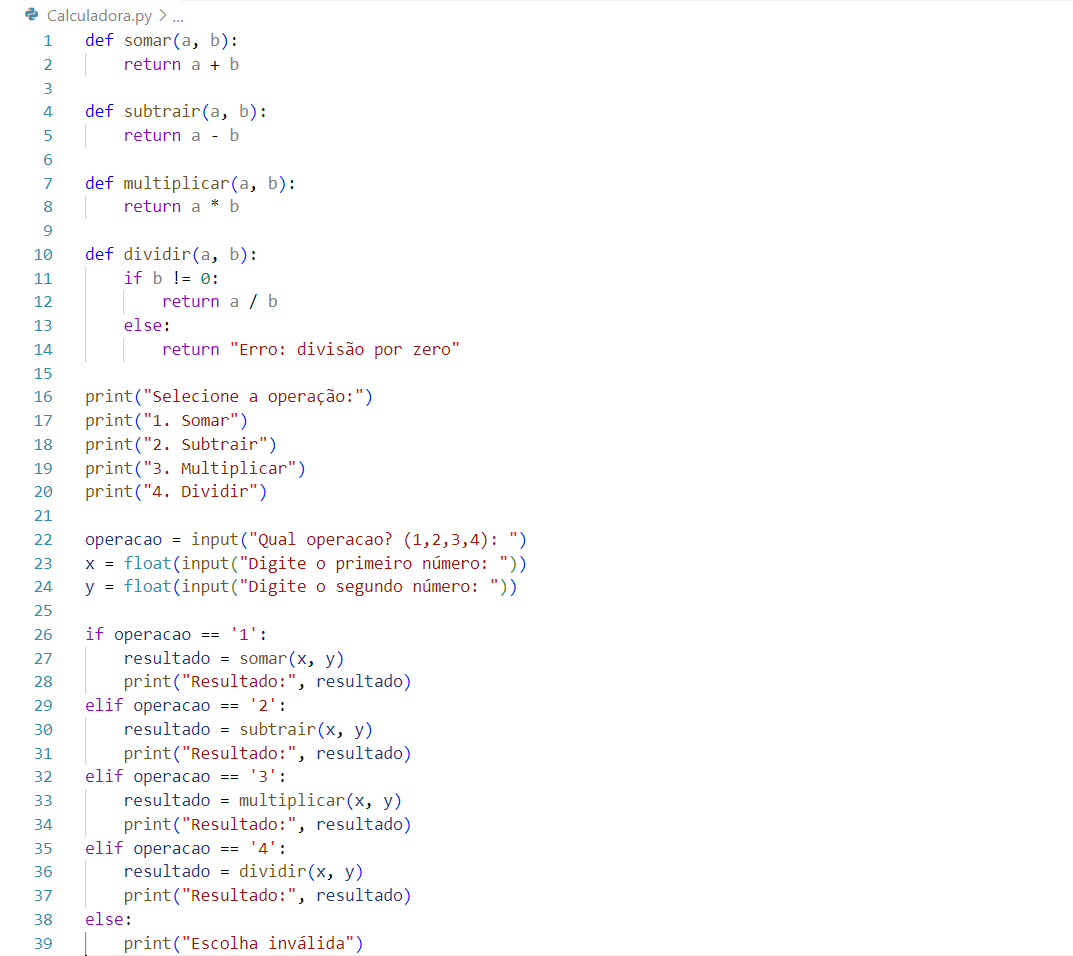
\includegraphics[width=12cm]{calculadora} 
    		\newline
    		Fonte: Criado por Mariana Cossetti Dalfior
    	\end{center}
    \end{figure}

 \begin{figure}[H]
	\begin{center}
		\caption{Resultado do c\'{o}digo fonte da calculadora} \label{resulcalc}
		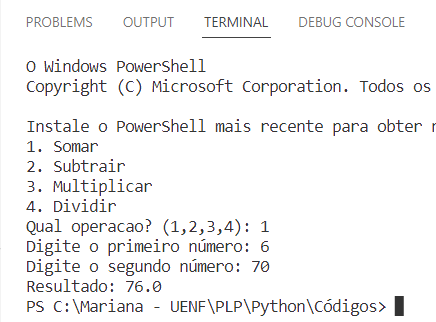
\includegraphics[width=9cm]{resulcalc} 
		\newline
		Fonte: Criado por Mariana Cossetti Dalfior
	\end{center}
\end{figure}

Al\'{e}m dessas opera\c{c}\~{o}es mostradas acima, existe a radicia\c{c}\~{a}o. Que possui uma fun\c{c}\~{a}o j\'{a} definida capaz de ser importada do m\'{o}dulo \textsl{math}. O c\'{o}digo fonte \ref{fonteraiz} dessa opera\c{c}\~{a}o e seu resultado \ref{resulraiz} ser\~{a}o apresentados a seguir:

\begin{lstlisting}
>>> import math
>>> 
>>> raiz = float(input("\nValor para descobrir a raiz quadrada: 
"))
>>> resultado =  math.sqrt(raiz)
>>> 
>>> print("\nO valor da raiz quadrada e: ", resultado)
\end{lstlisting}

    \begin{figure}[H]
	\begin{center}
		\caption{C\'{o}digo fonte da radicia\c{c}\~{a}o} \label{fonteraiz}
		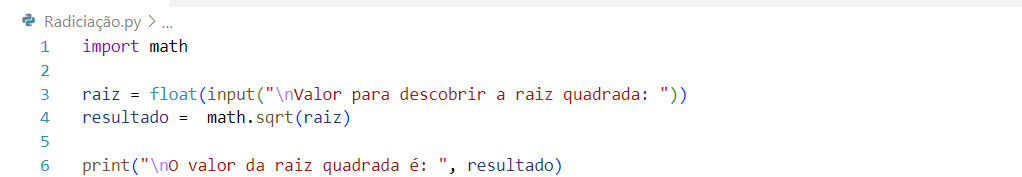
\includegraphics[width=15cm]{raiz} 
		\newline
		Fonte: Criado por Mariana Cossetti Dalfior
	\end{center}
\end{figure}

\begin{figure}[H]
	\begin{center}
		\caption{Resultado do c\'{o}digo fonte da radicia\c{c}\~{a}o} \label{resulraiz}
		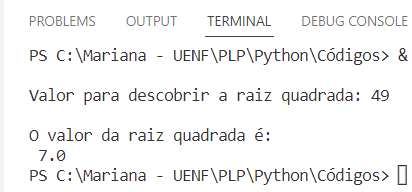
\includegraphics[width=9cm]{resulraiz} 
		\newline
		Fonte: Criado por Mariana Cossetti Dalfior
	\end{center}
\end{figure}

%%%=========================================================================================%%%
    \section{Programas com Objetos}
%%%=========================================================================================%%%
Para manipular dados em Python, \'{e} comum criar objetos que representem esses dados e facilitem sua manipula\c{c}\~{a}o. Existem diversas formas para a cria\c{c}\~{a}o de objetos e tamb\'{e}m diversas maneiras como, utilizando listas, matrizes, tuplas, dicion\'{a}rios, Pandas DataFrames, etc. Nessa aplica\c{c}\~{a}o foi criada duas classes e duas fun\c{c}\~{o}es para realizar a instancia\c{c}\~{a}o dessas classes, os quais recebem dois par\^{a}metros respons\'{a}veis pela defini\c{c}\~{a}o de atributos para os objetos. A seguir \'{e} poss\'{\i}vel observar o c\'{o}digo fonte \ref{objetos} e o resultado \ref{resulobjetos} da sua aplica\c{c}\~{a}o:
    
\begin{lstlisting}
>>> class Gato:
>>> def __init__(self, nome, idade):
>>> self.nome = nome
>>> self.idade = idade
>>> 
>>> class Dono:
>>> def __init__(self, nome, profissao):
>>> self.nome = nome
>>> self.profissao = profissao
>>> 
>>> gato = Gato("Auau", 1)
>>> dono = Dono("Mariana", "Estudante")
>>> 
>>> print("\nInformacoes do Cachorro:")
>>> print("Nome:", gato.nome)
>>> print("Idade:", gato.idade)
>>> print("\nInformacoes do Dono:")
>>> print("Nome:", dono.nome)
>>> print("Profissao:", dono.profissao)
\end{lstlisting}
    
\begin{figure}[H]
  	\begin{center}
  		\caption{C\'{o}digo fonte de Programa com Objetos} \label{objetos}
  		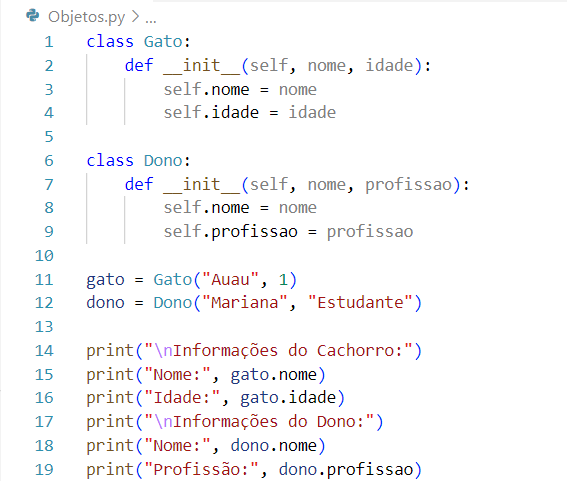
\includegraphics[width=10cm]{objetos} 
  		\newline
  		Fonte: Criado por Mariana Cossetti Dalfior
  	\end{center}
\end{figure}

\begin{figure}[H]
  	\begin{center}
  		\caption{Resultado do c\'{o}digo fonte de Programa com Objetos} \label{resulobjetos}
  		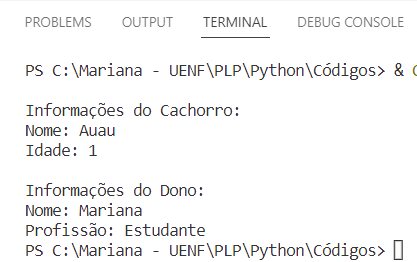
\includegraphics[width=8cm]{resulobjetos} 
  		\newline
  		Fonte: Criado por Mariana Cossetti Dalfior
  	\end{center}
\end{figure}
    

%%%=========================================================================================%%%
    \section{O algoritmo Quicksort}
%%%=========================================================================================%%%
O Quicksort \'{e} um algoritmo de ordena\c{c}\~{a}o com base no m\'{e}todo de divis\~{a}o e conquista, na etapa da divis\~{a}o \'{e} onde tudo realmente acontece. Na aplica\c{c}\~{a}o a seguir h\'{a} a ordena\c{c}\~{a}o de um vetor em ordem crescente, para isso o algoritmo come\c{c}a comparando todos os valores com o primeiro elemento. Ap\'{o}s isso h\'{a} a cria\c{c}\~{a}o de um subvetor para elementos menores que o primeiro e um outro subvetor para elementos maiores, ordenando esses novamente utilizando o quicksort na recursividade, e em seguida \'{e} inserido o primeiro elemento no seu devido lugar. A seguir \'{e} poss\'{\i}vel observar o c\'{o}digo fonte \ref{resulquicksort} da sua aplica\c{c}\~{a}o, retirados do livro \cite{Ramalho2022}: 

\begin{lstlisting}
>>> def quicksort(arr):
>>> if len(arr) <= 1:
>>> return arr
>>> else:
>>> pivot = arr[0]
>>> less = [x for x in arr[1:] if x <= pivot]
>>> greater = [x for x in arr[1:] if x > pivot]
>>> return quicksort(less) + [pivot] + quicksort(greater)
>>> 
>>> arr = [4, 2, 7, 1, 3]
>>> sorted_arr = quicksort(arr)
>>> print('\nVetor ordenado: ', sorted_arr)
\end{lstlisting}

\begin{figure}[H]
	\begin{center}
		\caption{C\'{o}digo fonte de Quicksort} \label{quicksort}
		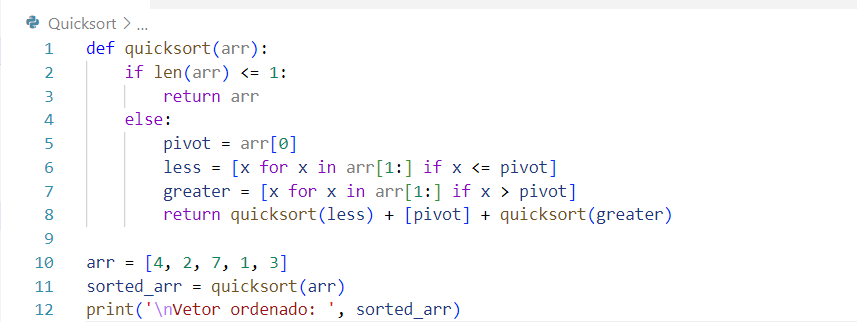
\includegraphics[width=12cm]{quicksort} 
		\newline
		Fonte: Exemplo 5.2
	\end{center}
\end{figure}

\begin{figure}[H]
	\begin{center}
		\caption{Resultado do c\'{o}digo fonte de Quicksort} \label{resulquicksort}
		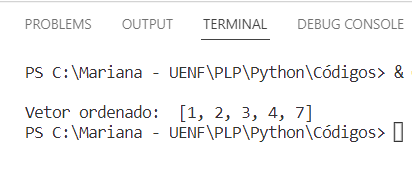
\includegraphics[width=6cm]{resulquicksort} 
		\newline
		Fonte: Exemplo 5.2
	\end{center}
\end{figure}

%%%=========================================================================================%%%
    \section{Aplica\c{c}\~{o}es com Banco de Dados}
%%%=========================================================================================%%%
A linguagem Python \'{e} amplamente utilizada para manipular bancos de dados e facilitar o estudo e an\'{a}lise desses dados. Python oferece v\'{a}rias maneiras de trabalhar com bancos de dados e oferece uma ampla gama de op\c{c}\~{o}es para cientistas de dados. Uma maneira \'{e} utilizar uma biblioteca padr\~{a}o chamada "\textsl{sqlite3}" que permite criar e manipular bancos de dados \textsl{SQLite}. Que \'{e} um banco de dados leve e amplamente utilizado, ideal para projetos menores ou aplica\c{c}\~{o}es que n\~{a}o exijam uma infraestrutura mais complexa. Nessa aplica\c{c}\~{a}o, \'{e} criada uma conex\~{a}o com um banco de dados, em seguida cria uma tabela e insere dados nela, ap\'{o}s isso esses dados s\~{a}o recuperados e impressos com o \textsl{print}. A seguir \'{e} poss\'{\i}vel observar o c\'{o}digo fonte \ref{bancodedados} e o resultado \ref{resulbancodedados} da sua aplica\c{c}\~{a}o, retirados do livro \cite{Guttag2021}: 

\begin{lstlisting}
>>> import sqlite3
>>> 
>>> conn = sqlite3.connect('exemplo7.2.db')
>>> 
>>> conn.execute('''CREATE TABLE IF NOT EXISTS clientes
>>> (id INTEGER PRIMARY KEY AUTOINCREMENT,
>>> nome TEXT NOT NULL,
>>> idade INTEGER NOT NULL);''')
>>> 
>>> conn.execute("INSERT INTO clientes (nome, idade) VALUES 
('Jose', 22)")
>>> conn.execute("INSERT INTO clientes (nome, idade) VALUES 
('Mariana', 20)")
>>> 
>>> cursor = conn.execute("SELECT * FROM clientes")
>>> 
>>> for row in cursor:
>>> print(f"ID: {row[0]}, Nome: {row[1]}, Idade: {row[2]}")
>>> 
>>> conn.close()
\end{lstlisting}

\begin{figure}[H]
	\begin{center}
		\caption{C\'{o}digo fonte de banco de dados} \label{bancodedados}
		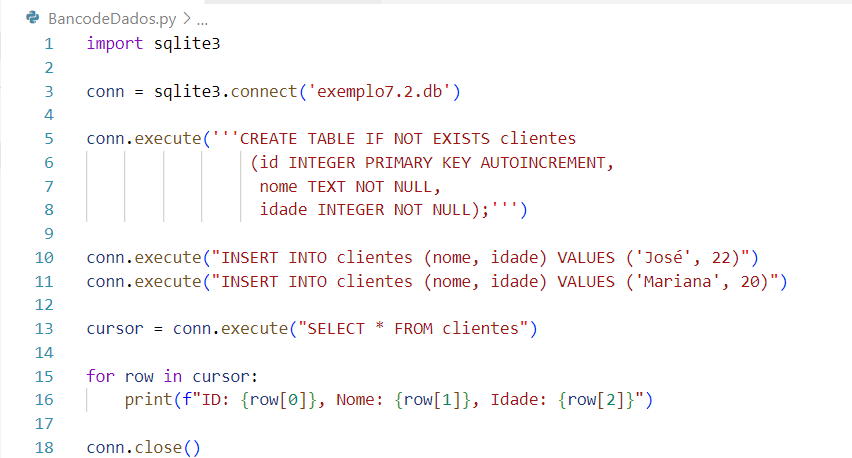
\includegraphics[width=12cm]{bancodedados} 
		\newline
		Fonte: Exemplo 7.2
	\end{center}
\end{figure}

\begin{figure}[H]
	\begin{center}
		\caption{Resultado do c\'{o}digo fonte de banco de dados} \label{resulbancodedados}
		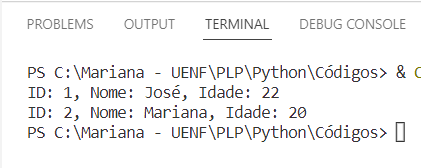
\includegraphics[width=8cm]{resulbancodedados} 
		\newline
		Fonte: Exemplo 7.2
	\end{center}
\end{figure}

%%%=========================================================================================%%%
\section{Programa de C\'{a}lculo Num\'{e}rico}
%%%=========================================================================================%%%

Em Python, o C\'{a}lculo Num\'{e}rico \'{e} um campo complexo e possui diversas bibliotecas que oferecem suporte \`{a} manipula\c{c}\~{a}o e an\'{a}lise de dados num\'{e}ricos. \'{E} not\'{a}vel nessas bibliotecas o \textsl{NumPy}, que fornece forte suporte para muitos programas e fun\c{c}\~{o}es matem\'{a}ticas, e tamb\'{e}m \textsl{SciPy}, que fornece recursos adicionais como a integra\c{c}\~{a}o, interpola\c{c}\~{a}o e otimiza\c{c}\~{a}o num\'{e}rica. Nessa aplica\c{c}\~{a}o para encontrar a ra\'{\i}z da fun\c{c}\~{a}o \'{e} aplicado de forma repetida o m\'{e}todo de bisse\c{c}\~{a}o, o qual vai atualizando o intervalo e verificando o crit\'{e}rio de parada. A seguir \'{e} poss\'{\i}vel observar o c\'{o}digo fonte \ref{calculonum} e o resultado \ref{resulcalcnum} da sua aplica\c{c}\~{a}o, retirados do livro \cite{Marcondes2018}:

\begin{lstlisting}
>>> def calcula_f(x):
>>> return x ** 3 + 5 * x ** 2 - 5 * x - 12
>>> 
>>> iteracao_maxima = 100
>>> 
>>> iteracao = 0
>>> 
>>> erro_definido = 0.0001
>>> 
>>> parar = 0
>>> 
>>> a = -6.0  
>>> b = -4.0  
>>> 
>>> y1 = calcula_f(a)  
>>> y2 = calcula_f(b) 
>>> 
>>> x0_anterior = 2*b
>>> 
>>> if y1 * y2 > 0:
>>> print (u'erro de Execucao - Redefinir valores de a e b.')
>>> else:
>>> while parar == 0:
>>> iteracao = iteracao + 1  
>>> x0 = (a + b) / 2  
>>> y0 = calcula_f(x0)  
>>> 
>>> if y1 * y0 > 0:
>>> a = x0  
>>> 
>>> if y2*y0 > 0:
>>> b = x0  
>>> 
>>> erro = abs(x0 - x0_anterior)
>>> 
>>> x0_anterior = x0  
>>> 
>>> if (iteracao > iteracao_maxima) or (erro < erro_definido):
>>> parar = 1
>>> 
>>> print (u'\nTotal de Iteracoes')
>>> print (iteracao)
>>> 
>>> print ('\nValor de x')
>>> print ('x = ', x0)
>>> 
>>> print ('\nerro encontrado')
>>> print ('erro = ', erro)
\end{lstlisting}

\begin{figure}[H]
	\begin{center}
	\caption{C\'{o}digo fonte de C\'{a}lculo Num\'{e}rico} \label{calculonum}
	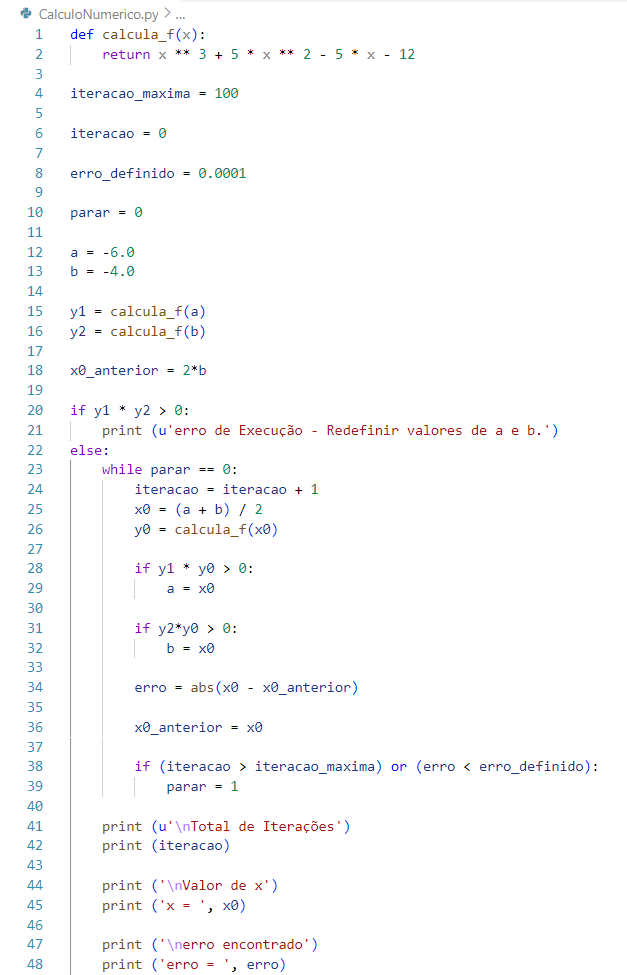
\includegraphics[width=12cm]{calculonum} 
	\newline
	Fonte: Exemplo 9.1 do livro
	\end{center}
\end{figure}

\begin{figure}[H]
	\begin{center}
	\caption{Resultado do c\'{o}digo fonte de C\'{a}lculo Num\'{e}rico} \label{resulcalcnum}
	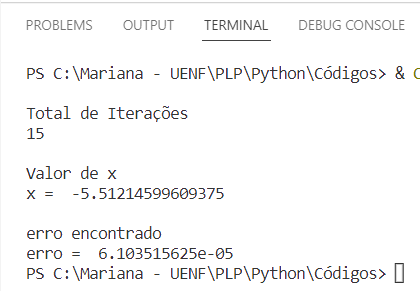
\includegraphics[width=9cm]{resulcalcnum} 
	\newline
	Fonte: Exemplo 9.1 do livro
	\end{center}
\end{figure}